\documentclass[12pt, oneside]{report}

\usepackage[utf8]{inputenc} % Required for inputting international characters
\usepackage[T1]{fontenc} % Output font encoding for international characters
\usepackage[a4paper,left=1in,right=1in,top=.75in,bottom=.75in]{geometry}
\usepackage{mathpazo} % Palatino font
\usepackage{graphicx}
\usepackage{sectsty}
\usepackage{epigraph}
\usepackage{indentfirst}
\usepackage{float}
\usepackage[pagestyles]{titlesec}
\usepackage{setspace}
\usepackage[nottoc,notlof,notlot]{tocbibind}
\usepackage{listings}
\usepackage[hidelinks]{hyperref}
\usepackage{amsmath,bm} 
\usepackage{subfig}
\usepackage{etoolbox}
\usepackage{amssymb}


% correct a bug in titlesec package
\makeatletter
\patchcmd{\ttlh@hang}{\parindent\z@}{\parindent\z@\leavevmode}{}{}
\patchcmd{\ttlh@hang}{\noindent}{}{}{}
\makeatother
% \renewcommand{\baselinestretch}{1.5} 
\makeatletter\renewcommand*\l@part[2]{}\makeatother
\renewcommand\bibname{References}
\titleformat{\chapter}[display]
{\normalfont\Large\bfseries}{\scshape\chaptertitlename\ \thechapter}{20pt}{\filcenter\LARGE\scshape}
\titleformat{\part}
{\filcenter\thispagestyle{empty}\addtocounter{page}{-1}\normalfont\Large\bfseries}{}{20pt}{\filcenter\Huge\scshape}
\titleformat{\section}{\bfseries\large}{\thesection}{0.4em}{}
\titleformat{\subsection}{\bfseries}{\thesubsection}{0.4em}{}


\titlespacing*{\chapter}{0pt}{0pt}{20pt}
% \titleformat*{\subsection}{\bfseries}
\setlength\epigraphwidth{.8\textwidth}
\setlength\epigraphrule{1pt}


\newpagestyle{fncy}{
  \setheadrule{.4pt}
  \setfootrule{.4pt}% Header rule
  \sethead[Image Regeneration with Generative Models]% odd-left
          []% odd-center
          [\chaptertitle]% odd-right
          {Image Regeneration with Generative Models}% even-left
          {}% even-center
          {\chaptertitle}% even-right
  \setfoot[Department of CSE, Sir MVIT]% odd-left
          []% odd-center
          [\thepage]% odd-right
          {Department of CSE, Sir MVIT}% even-left
          {}% even-center
          {\thepage}% even-right
}

\pagestyle{plain}


\begin{document}

%----------------------------------------------------------------------------------------
{\setstretch{1.0}

%----------------------------------------------------------------------------------------
%	TITLE PAGE
%----------------------------------------------------------------------------------------

\begin{titlepage} % Suppresses displaying the page number on the title page and the subsequent page counts as page 1
	\newcommand{\HRule}{\rule{\linewidth}{0.5mm}} % Defines a new command for horizontal lines, change thickness here

	\center % Centre everything on the page

	%------------------------------------------------
	%	Headings
	%------------------------------------------------
	\textsc{\LARGE Visvesvaraya Technological University\\[3pt]Belgaum 590014}\\[10pt] 
	%------------------------------------------------
	%	Logo
	%------------------------------------------------
	
\includegraphics[width=0.15\textwidth]{images/vtu.png}\\[10pt] 

	{\Large Synopsis Entitled}\\[10pt] % Major heading such as course name

	%------------------------------------------------
	%	Title
	%------------------------------------------------

	\HRule\\[10pt]
	\textsc{\huge \textbf{Image Regeneration With Generative}\\[3pt] \textbf{Models}}\\[10pt]

	\HRule\\[10pt]
	\Large{
		Submitted for\\
		\textbf{Bachelor Of Engineering}\\
		In \\
		\textbf{Computer Science And Engineering} \\
		For the Academic year 2017-2018 
	}\\[15pt]
	\Large{Submitted by}\\[2pt]
	%------------------------------------------------
	%	Author(s)
	%------------------------------------------------
	\begin{tabular}{ l r }
		\textsc{\Large \textbf{Abhijith C.}}       & \Large \textbf{1MV14CS004} \\
		\textsc{\Large \textbf{Raghava G. Dhanya}} & \Large \textbf{1MV14CS077} \\
		\textsc{\Large \textbf{Shashank S.}}       & \Large \textbf{1MV14CS131}
	\end{tabular}\\[15pt]

	\Large{Project carried out at\\
		\textbf{Sir M. Visvesvaraya Institute of Technology}
		\\Bangalore-562157
	}\\[10pt]
	\Large{Under the Guidance of\\
		\textbf{\textsc{\Large Mrs. Sushila Shidnal }}\\
		Assistant Professor, Department of CSE\\
		Sir M Vivesvaraya Institute of Technology, Bangalore.
	}\\[10pt]
	%------------------------------------------------
	%	Logo
	%------------------------------------------------
	
\includegraphics[width=0.15\textwidth]{images/mvit.png}\\[10pt] 
	\Large{
		\textbf{Department Of Computer Science \& Engineering}\\
		\textbf{Sir M. Visvesvaraya Institute Of Technology}\\
		Hunasamaranahalli, Bangalore-56215\\
	}

\end{titlepage}

\par

%----------------------------------------------------------------------------------------
%	TITLE PAGE
%----------------------------------------------------------------------------------------

\begin{titlepage} % Suppresses displaying the page number on the title page and the subsequent page counts as page 1
	\newcommand{\HRule}{\rule{\linewidth}{0.5mm}} % Defines a new command for horizontal lines, change thickness here

	\center % Centre everything on the page

	%------------------------------------------------
	%	Headings
	%------------------------------------------------
	\textsc{\LARGE Visvesvaraya Technological University\\[3pt]Belgaum 590014}\\[10pt] 
	%------------------------------------------------
	%	Logo
	%------------------------------------------------
	
\includegraphics[width=0.15\textwidth]{images/vtu.png}\\[10pt] 

	{\Large Synopsis Entitled}\\[10pt] % Major heading such as course name

	%------------------------------------------------
	%	Title
	%------------------------------------------------

	\HRule\\[10pt]
	\textsc{\huge \textbf{Image Regeneration With Generative}\\[3pt] \textbf{Models}}\\[10pt]

	\HRule\\[10pt]
	\Large{
		Submitted for\\
		\textbf{Bachelor Of Engineering}\\
		In \\
		\textbf{Computer Science And Engineering} \\
		For the Academic year 2017-2018 
	}\\[15pt]
	\Large{Submitted by}\\[2pt]
	%------------------------------------------------
	%	Author(s)
	%------------------------------------------------
	\begin{tabular}{ l r }
		\textsc{\Large \textbf{Abhijith C.}}       & \Large \textbf{1MV14CS004} \\
		\textsc{\Large \textbf{Raghava G. Dhanya}} & \Large \textbf{1MV14CS077} \\
		\textsc{\Large \textbf{Shashank S.}}       & \Large \textbf{1MV14CS131}
	\end{tabular}\\[15pt]

	\Large{Project carried out at\\
		\textbf{Sir M. Visvesvaraya Institute of Technology}
		\\Bangalore-562157
	}\\[10pt]
	\Large{Under the Guidance of\\
		\textbf{\textsc{\Large Mrs. Sushila Shidnal }}\\
		Assistant Professor, Department of CSE\\
		Sir M Vivesvaraya Institute of Technology, Bangalore.
	}\\[10pt]
	%------------------------------------------------
	%	Logo
	%------------------------------------------------
	
\includegraphics[width=0.15\textwidth]{images/mvit.png}\\[10pt] 
	\Large{
		\textbf{Department Of Computer Science \& Engineering}\\
		\textbf{Sir M. Visvesvaraya Institute Of Technology}\\
		Hunasamaranahalli, Bangalore-56215\\
	}

\end{titlepage}

\par
}
\begin{titlepage}
\begin{center}
\noindent\textsc{\textbf{\Large Sir M Visvesvaraya Institute of Technology}}\\[3pt]
\textsc{\textbf{\large Bengaluru 562157\\[3pt]Department of Computer Science and Engineering}}\\[15pt]

\includegraphics[width=0.2\textwidth]{images/mvit.png}\\[15pt] 
\textsc{\textbf{\Large Certificate}}\\
\end{center}
This is to certify that the project work entitled "Image Regeneration With Generative Models" has been carried out by Abhijith C. (1MV14CS004), Raghava G. Dhanya (1MV14CS077) and Shashank S. (1MV14CS131), bona-fide students of Sir M Visvesvaraya Institute of Technology, in partial fulfillment for the award of the Degree of Bachelor of Engineering in Computer Science and Engineering of the Visvesvaraya Technological University, Belagavi during the year 2016-2017. It is certified that all corrections and suggestions indicated during Internal Assessment have been incorporated into the report deposited in the department library. The project report has been approved as it satisfies the academic requirements with respect to the project work prescribed for the course of Bachelor of Engineering.

\vspace{100px}

\noindent
\begin{tabular*}{\textwidth}{@{} l @{\extracolsep{\fill}} l @{\extracolsep{\fill}} l @{}}
    \textsc{\textbf{\small Mrs. Sushila Shidnal}} & \textsc{\textbf{\small Prof. Dilip K Sen}}  & \textsc{\small \textbf{Dr. V. R. Manjunath}}\\
    \textbf{\small Asst. Prof \& Internal Guide}   & \textbf{\small Head of Department} & \textbf{\small Principal}\\
    \textbf{\small Dept. of CSE, Sir MVIT}        & \textbf{\small Dept. of CSE, Sir MVIT}           &  \textbf{\small Sir MVIT}
\end{tabular*}\\[35pt]
\textbf{Name of the examiners}\hfill\textbf{Signature with date}\\
1)\\
2)
\end{titlepage}\par
\begin{titlepage}

% \chapter*{Declaration}
\
\begin{center}
\normalfont\LARGE\textbf{\textsc{Declaration}}\\[20pt]
\end{center}
We hereby declare that the entire project work embodied in this dissertation has been carried out by us and no part has been submitted for any degree or diploma of any institution previously.\bigskip\\

\noindent Place: Bengaluru\\
Date:\\

\vspace{200px}
\noindent
\begin{tabular*}{\textwidth}{@{} l @{\extracolsep{\fill}} l @{\extracolsep{\fill}} l @{}}
    \textsc{\textbf{\small Abhijith C.}} & \textsc{\textbf{\small Raghava G. Dhanya}}  & \textsc{\small \textbf{Shashank S.}}\\
    \textbf{\small 1MV14CS004}   & \textbf{\small 1MV14CS077} & \textbf{\small 1MV14CS131}
\end{tabular*}\\[35pt]
\vspace{100px}

\end{titlepage}

\par
\chapter*{Acknowledgments}
\noindent This project would not have been possible without the contributions of many people.\par\bigskip
We are pleased to express our sincere thanks to the administration of the \textbf{Sir M. Visvesvaraya Institute of Technology}, Bangalore, which has given us the opportunity and the resources to carry out our projects in their facilities.\par\bigskip
We would also like to convey our sincere thanks \textbf{Dr. V. R. Manjunath}, principal, Sir MVIT for providing us with the infrastructure and facilities needed to develop our project.\par\bigskip
We would like to thank the \textbf{Prof Dilip K. Sen}, Head of the department, CSE, Sir MVIT for providing an intellectual environment where we could devote a tremendous amount of time to work on this project.\par\bigskip
We wish to express our heartfelt gratitude to our guide, \textbf{Smt. Sushila Shidnal}, for her invaluable guidance, encouragement, support and advice.\par\bigskip
We thank \textbf{Google} for \textbf{Google colaboratory} where we ran most of our Deep Learning model training.\par\bigskip
Our immense gratitude for the members of faculty of \textbf{Department of Computer Science and Engineering}, Sir MVIT for support and co-operation. Lastly we thank all our friend for their help and suggestion without which this project would not have been possible.\par\bigskip
\vspace{50px}
\noindent\hfill\begin{tabular}{ l r }
        \textsc{-  \textbf{Abhijith C.}}       &  \textbf{1MV14CS004} \\
        \textsc{-  \textbf{Raghava G. Dhanya}} &  \textbf{1MV14CS077} \\
        \textsc{-  \textbf{Shashank S.}}       &  \textbf{1MV14CS131}
\end{tabular}\par

\pagenumbering{roman}
\chapter*{Abstract\markboth{Abstract}{Abstract}}\label{ch:abstract}
\addcontentsline{toc}{chapter}{Abstract}

Current advances in Generative Adversial Networks allow us to obtain near realistic images of faces but it is still quite distinguishable from actual photographic images. The technology is also not very amiable to changes in the orientation of faces in Convolutional Neural Networks(CNN). Additionally, the amount of data required to train the network must be exhaustible, for example, in case different perspectives of a face are required the various perspectives must be explicitly present in the training data to achieve the result. Thus the network requires humongous amounts of data.
\par\bigskip
In this paper we propose a novel approach to accomplish the same results using CapsNet. CapsNet employs a dynamic routing algorithm which replaces the scalar-output feature detectors of the CNN with vector-output capsules. A capsule is essentially a group of neurons describing a specific part of obect or image. Active capsules at one level make predictions, via transformation matrices, for the instantiation parameters of
higher-level capsules. In essence, the CapsNet is the reverse of the common Computer Graphics pipeline where we convert objects to their renders. The CapsNet works from the pixel level and works up towards the object.
\par\bigskip
We propose that the amount of data required to train a comparable model is very small while it gives comparable, if not better, results. \par
\tableofcontents
\listoffigures
\clearpage
\pagenumbering{arabic}
% \pagestyle{plain}
\renewpagestyle{plain}{
  \setheadrule{.4pt}
  \setfootrule{.4pt}% Header rule
  \sethead[Image Regeneration with Generative Models]% odd-left
          []% odd-center
          [\chaptertitle]% odd-right
          {Image Regeneration with Generative Models}% even-left
          {}% even-center
          {\chaptertitle}% even-right
  \setfoot[Department of CSE, Sir MVIT]% odd-left
          []% odd-center
          [\thepage]% odd-right
          {Department of CSE, Sir MVIT}% even-left
          {}% even-center
          {\thepage}% even-right
}
\pagestyle{fncy}

\part*{Chapter 1\\ Introduction}
\chapter{Introduction}\label{ch:introduction}

\epigraph{\textit{\Large "What I cannot create, I do not understand."}}{\textit{ \Large Richard Feynman}}
One of the main aspirations of Artificial Intelligence is to develop algorithms and techniques that enrich computers with ability to understand our world. Generative models are one of the most promising approaches towards achieving this goal.\par\bigskip
A generative model is a mathematical or statistical model to generate all values of a phenomena. To train such a model, we first collect a large amount of data in some domain (e.g., think millions of images, sentences, or sounds, etc.) and then train a model to generate data like it.\par\bigskip
A generative algorithm models how data was generated to classify a signal. It poses the question: according to my generation hypotheses, which category is most likely to generate this signal? A discriminant algorithm does not care about how the data was generated, it just classifies a given signal. A generative model learns the joint probability distribution $p(x,y)$ while a discriminative model learns the conditional probability distribution $p(y|x)$ “probability of y given x”.\par\bigskip
The trick is that the neural networks that we use as generating models have a significantly smaller number of parameters than the amount of data on which we train them, so the models are forced to effectively discover and internalize the essence of the data to generate it.\par\bigskip
There are multiple approaches to build a generative models
\begin{itemize}
  \item Generative adversarial networks (GANs) are a class of generative algorithms used in unsupervised machine learning, implemented by a system of two neural networks competing in a zero-sum game framework. They were presented by Ian Goodfellow et al. in 2014 [1]. This technique can generate photographs that seem at least superficially authentic to human observers, having many realistic features (though in tests people can tell real from generated in many cases).
  \item Variational Autoencoders (VAEs) allow us to formalize this problem in the framework of probabilistic graphical models where we are maximizing a lower bound on the log likelihood of the data
  \item Autoregressive models such as PixelRNN, on the other hand train a network that models the conditional distribution of every individual pixel given previous pixels (to the left and to the top). This is similar to plugging the pixels of the image into a char-rnn, but the RNNs runs both horizontally and vertically over the image instead of just a 1D sequence of characters.
\end{itemize} \par
Generative Adversarial Networks, which we already discussed above, pose the training process as a game between two distinct networks: a generator network (as seen above) and a second discriminative network that tries to classify samples as either coming from the true distribution $p(x)$ or the model distribution $\hat{p}(x)$. Every time the discriminator notices a difference between the two distributions the generator adjusts its parameters slightly to make it go away, until at the end (in theory) the generator exactly reproduces the true data distribution and the discriminator is guessing at random, unable to find a difference.

% \section{Some section}
% blah blah blah
% \subsection{some subsection}
% blah blah
\par

\part*{Chapter 2\\ Literature Survey}
\chapter{Literature Survey}\label{ch:literature_survey}
\epigraph{\textit{\Large “Adversarial training is the coolest thing since sliced bread”}}{\textit{ \large Yann LeCun,\\ Director of AI Research at Facebook and Professor at NYU}}
GANs were first introduced by Ian Goodfellow et al. in 2014[1] in Neural Information Processing Systems 2014 (NIPS 2014). The paper proposes a completely new framework for estimating generative models via an adversarial process. In this process two models are simultaneously trained. According to [1] the network has a generative model G that captures the data distribution, and a discriminative model D that estimates the probability that a sample came from the training data rather than G. This framework corresponds to a minimax two-player game. There is no need for any Markov chains or unrolled approximate inference networks during either training or generation of samples. This original work by Ian Goodfellow uses fully connected neural networks in the generator and the discriminator.\par\bigskip
\begin{figure}[H]
\centering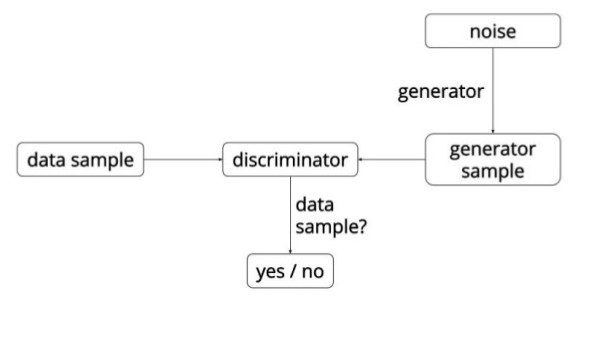
\includegraphics[width=.7\textwidth]{images/vanilaGAN.jpg}
\caption{Vanilla Generative Adversarial Network}
\end{figure}
Since then, there has been tremendous advancements in Deep Learning. A convolutional neural network (CNN, or ConvNet) [2] is a class of deep, feed-forward artificial neural networks that has successfully been applied to analyzing visual imagery. These networks uses convolution layers in its core. The convolution layer's parameters consist of a set of learnable filters, also called as kernels, which have a small receptive field, but they extend through the full depth of the input volume. During the forward pass, each filter is convolved across the width and height of the input volume, computing the dot product between the entries of the filter and the input and producing a 2-dimensional activation map of that filter. As a result, the network learns filters that activate when it detects some specific type of feature at some spatial position in the input.\par\bigskip
\begin{figure}[H]
\centering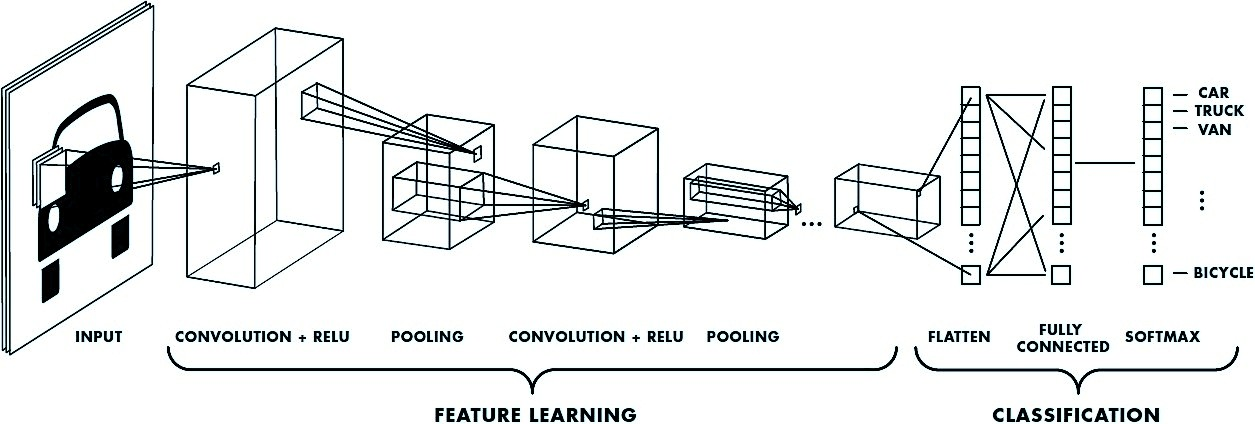
\includegraphics[width=.7\textwidth]{images/CNN.jpg}
\caption{Convolutional Neural Network}
\end{figure}
A breakthrough development that occurred in Adversarial Networks was the introduction of “Deep Convolutional Generative Adversarial Networks” by Alec Radford et al, ICLR, 2016 in 2016 in ICLR[3]. He applied a list of empirically validated tricks as the substitution of pooling and fully connected layers with convolutional layers.\par\bigskip
\begin{figure}[H]
\centering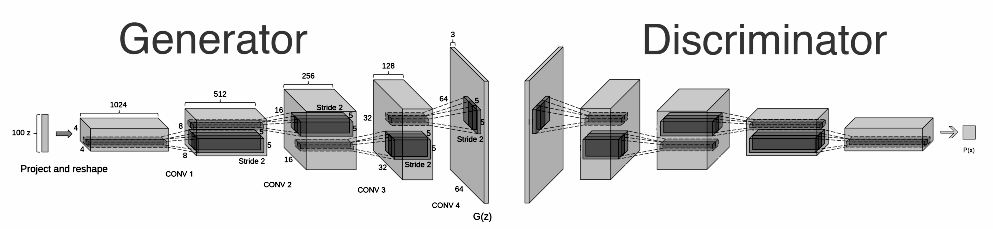
\includegraphics[width=1\textwidth]{images/dcgan.png}
\caption{Deep Convolutional Generative Adversarial Network}
\end{figure}
The power of the features encoded in the latent variables was further explored by Chen at al. [4]. They made use of the fact that the latent space of a regular GAN is underspecified to add additional input parameters (referred to as extend code) and thereby functionality. They decomposed the code in the latent code seen before and an additional latent component, which targets the semantic features of the data distribution. The goal is to learn disentangled and interpretable representations.\par\bigskip
Today, most GANs are loosely based on the former shown DCGAN [3] architecture. Many papers have focused on improving the setup to enhance stability and performance. Many key insights was given by Salimans et al.[5]:
\begin{itemize}
\item Usage of convolution with stride instead of pooling
\item Usage of Virtual Batch Normalization
\item Usage of Minibatch Discrimination in DD
\item Replacement of Stochastic Gradient Descent with Adam Optimizer [6]
\item Usage of one-sided label smoothing
\end{itemize}
Another huge development came with the introduction of Wasserstein GANs by Martin Arjovsky [7] . He introduced a new algorithm named WGAN, an alternative to traditional GAN training. In this new model, he showed that the stability of learning can be improved, remove problems like mode collapse, and provide good learning curves useful for debugging and hyperparameter searches.\par\bigskip
This recently proposed Wasserstein GAN (WGAN) makes progress toward stable training of GANs, but sometimes can still generate only low-quality images or fail to converge. 
Ishaan Gulrajani with Martin Arjovsky proposed an alternative in [8] to fix the issues the previous GAN faced. This proposed method performs better than standard WGAN and enables stable training of a wide variety of GAN architectures with almost no hyperparameter tuning, including 101-layer ResNets[9] and language models over discrete data.\par\bigskip
A big breakthrough in the field of Deep Learning came with the introduction of CapsNets or Capsule Networks[10] by the Godfather of Deep Learning, Geoffrey Hinton. CNNs perform exceptionally great when they are classifying images which are very close to the data set. If the images have rotation, tilt or any other different orientation then CNNs have poor performance. This problem was solved by adding different variations of the same image during training.\par\bigskip
\bigskip
\begin{figure}[H]
\centering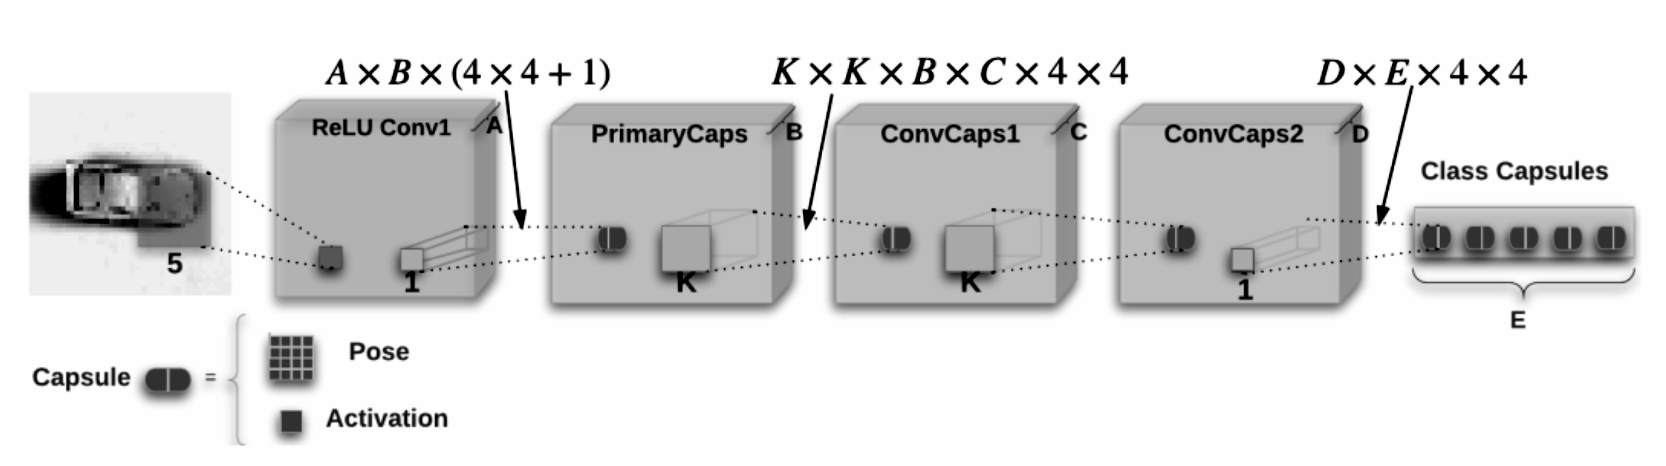
\includegraphics[width=1\textwidth]{images/caps.png}
\caption{Capsule Network}
\end{figure}
The key features of this breakthrough are Layer based Squashing and Dynamic Routing.
In a typical Convolutional Neural Network, the squashing function is added to each layer of the CNN model. A squashing function compresses the input to one of the ends of a small interval, introducing nonlinearity to the neural network and enables the network to be effective. Whereas, in a Capsule network, the squashing function is applied to the vector output of each capsule.\par\bigskip
Instead of applying non-linearity to each neuron, the squashing function applies squashing to a group of neurons i.e the capsule. To be more precise, it applies nonlinearity to the vector output of each capsule. The squashing function also tries to squash the vector output to zero if it is a small vector. If the vector is too long, the function tries to limit the output vector to 1.\par\bigskip
Dynamic routing algorithm in CapsNet replaces the scalar-output feature detectors of the CNN with the vector-output capsules. Also, the max pooling feature in CNNs, which led to positional invariance, is replaced with ‘routing by agreement’. The algorithm ensures that when they forward propagate the data, it goes to the next most relevant capsule in the layer above. Although dynamic routing adds an extra computational cost to the capsule network, it has been proved to be advantageous to the network by making it more scalable and adaptable.

\par

\part*{Chapter 3\\ Technology}
\chapter{Technology}\label{ch:technology}
\epigraph{\textit{\Large “I think, therefore I am”}}{\textit{ \large René Descartes,\\ French philosopher and scientist}}
\begin{itemize}
	\item\textbf{Adversarial Training:} Two models undergoing training simultaneously by competing against each other. The output of each model acts as an adversary for the other to improve upon.
	\item\textbf{Generative Model:} Any model capable of generating completely new realistic data of a class.
	\item\textbf{Discriminative Model:} Here, as a Discriminator, a model which is capable of distinguishing between actual ground truth from the true distribution and generated information from a model.
	\item\textbf{Gradient Descent:} A method of optimizing an objective function using a first-order iterative approach to find a local minimum.
	\item\textbf{Gaussian Model:} A model that fits the data in the shape of a Gaussian function, identified by a characteristic "bell curve". CapsNet uses this to find agreeing probability outputs of the "capsules".
	\item\textbf{TensorFlow:} An open source software library for numerical computation using data flow graphs. It was originally developed by the Google Brain Team within Google's Machine Intelligence research organization for machine learning and deep neural networks research.

\end{itemize}

\textbf{\Large Other essentials:}

\begin{itemize}
	\item\textbf{CPU:} 3GHz quad core, x86-64 architecture (or)
	\item\textbf{GPU:} NVIDIA or any other TensorFlow supported GPU, CUDA or cuDNN
	\item\textbf{Python:} 2.7 or 3.4 and above
\end{itemize}

\par


\part*{Chapter 4\\ System Requirements}
\chapter{System Requirements}\label{ch:system_requirements}
\epigraph{\textit{\normalsize “Any A.I. smart enough to pass a Turing test is smart enough to know to fail it.”}}{\textit{ \normalsize Ian McDonald,\\ River of Gods}}

\section{Functional Requirements} % (fold)
\label{sec:functional_requirements}
The system must, at the minimum, fulfill certain basic requirements.
\begin{enumerate}
    \item Take a latent space vector or noise as input.
    \item Learn joint probability distribution of training images.
    \item Generate a realistic image of the training distribution that doesn't belong to training set.
    \item Use a binary Capsule network classifier to differentiates real or fake image.
\end{enumerate}
% section functional_requirements (end)
\section{Non Functional Requirements} % (fold)
\label{sec:non_functional_requirements}
The system should have following non functional requirements. These specify the quality of the system.
\begin{enumerate}
    \item Efficient, Fast forward and backward propagation.
    \item Curb data usage while maintaining high quality results.    
\end{enumerate}
% section non_functional_requirements (end)

\section{Development Requirement} % (fold)
\label{sec:development_requirement}
System requirements for training and demonstrating of the models
\subsection{Training System Requirements} % (fold)
\label{sub:training_system_requirements}
For training the model,
\begin{enumerate}
    \item python 3.4 or above
    \item Tensorflow 1.7 or above
    \item Keras  2.1.6 or above
    \item Numpy, Scipy, Matplotlib
    \item OpenCV 2
    \item CPU 1.6 GHz or above
    \item Nvdia GPU with CUDA compatibility 3.5 or above
    \item RAM 8GB or above
    \item Disk storage 20GB or above
\end{enumerate}
% subsection training_system_requirements (end)

\subsection{Demonstration System Requirements} % (fold)
\label{sub:demonstration_system_requirements}
For evaluating the model or just forward-propagation,
\begin{enumerate}
    \item python 3.4 or above
    \item Flask
    \item Browser - Google Chrome
    \item Tensorflow 1.7 or above
    \item Keras  2.1.6 or above
    \item Numpy, Scipy, Matplotlib
    \item OpenCV 2
    \item CPU 1 GHz or above
    \item RAM 4GB or above
    \item Disk storage 20GB or above
\end{enumerate}
% section development_requirement (end)
\par

\part*{Chapter 5\\ Proposed Architecture}
\chapter{Proposed Architecture}\label{ch:proposed_architecture}
\epigraph{\textit{\normalsize “Artificial intelligence, in fact, is obviously an intelligence transmitted by conscious subjects, an intelligence placed in equipment.”}}{\textit{ \normalsize Pope Benedict XVI}}

\section{Generator} % (fold)
\label{sec:generator}
We use a deep convolutional generator model, which is similar to what DCGAN uses as generator. It starts with a latent vector or noise of shape 100 which connects to a densely connected neural layer. We then use Reshape layer which reshapes it to an (8, 8, 128) matrix and which is then sent to the batch normalization layer. We later perform up-sampling by using DeConv (De-Convolutional layer: transposed convolutional layer) layer. DeConv layer is internally implemented by an up-sampling layer and a convolutional layer. We perform DeConv two more times to get the shape of the image as expected, which should be (64, 64, 3), which stands for a 64x64 RGB image.
\begin{figure}[H]
\centering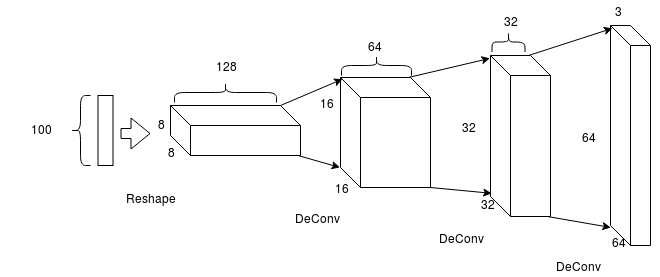
\includegraphics[width=1\textwidth]{images/Generator.png}
\caption{Generator architecture}
\label{fig:generator}
\end{figure} 

% section generator (end)


\section{Discriminator} % (fold)
\label{sec:discriminator}
The discriminator in the original models is replaced by our modification of CapsNet. We use a binary classifier CapsNet to distinguish between real and fake images. 

\par\bigskip
The CapsNet has 2 parts: encoder and decoder. The first 3 layers are encoder, and the second 3 are decoder:

Layer 1. Convolutional layer
Layer 2. PrimaryCaps layer
Layer 3. DigitCaps layer
Layer 4. Fully connected \#1
Layer 5. Fully connected \#2
Layer 6. Fully connected \#3

In our implementation, we do not use the decoder layers as we do not need the reconstruction aspects of the network for classification. Hence only the encoder layers are used.
\par\bigskip
The encoding part of the network takes as input a digital image of 64x64 and learns to encode it into a vector of 16 dimensions of instantiation parameters, this is where the capsules do their job. The output of the network during prediction is a 10-dimensional vector of the lengths of the DigitCaps' outputs.

% Discriminator image

\subsection{Layer 1: Convolutional Layer} % (fold)
\label{sub:layer_1_convolutional_layer}
\noindent Input: 64x64 image (three color channel).
\\Output: 56x56x256 tensor.
\\Number of parameters: 62464.

\par\bigskip The work of the convolutional layer consists of detecting the basic functions in the 2D image. In the CapsNet system, the convolutional layer has 256 kernels of size 9x9x1 and stride of 1, followed by the activation function, ReLU. To calculate the number of parameters, we must also remember that each kernel in a convolutional layer has 1 bias term. Therefore, this layer has (9 x 9 x 3 x 256 + 256 =) 62464 trainable parameters in total.

% subsection layer_1_convolutional_layer (end)

\subsection{Layer 2: PrimaryCaps Layer} % (fold)
\label{sub:layer_2_primarycaps_layer}
\noindent Input: 56x56x256 tensor.
\\Output: 24x24x8x32 tensor.
\\Number of parameters: 5308672.

\par\bigskip This layer has 32 primary capsules whose job is to take basic features detected by the convolutional layer and produce combinations of the features. The layer has 32 “primary capsules” that are very similar to convolutional layer in their nature. Each capsule applies eight 9x9x256 convolutional kernels to the 56x56x256 input volume and therefore produces 24x24x8 output tensor. Since there are 32 such capsules, the output volume has shape of 24x24x8x32. Doing calculation similar to the one in the previous layer, we get (9 x 9 x 256 x 256 + 256 =) 5308672 trainable parameters in this layer.

% subsection layer_2_primarycaps_layer (end)

\subsection{Layer 3: DigitCaps Layer} % (fold)
\label{sub:layer_3_digitcaps_layer}
\noindent Input: 24x24x8x32 tensor.
\\Flattened to: 147456
\\Output: 1x1 matrix.
\\Number of parameters: 1497600.

\par\bigskip We have a 3 hidden-layer densely connected neural network which takes the flattened input to give a binary classification output of 1x1. Each hidden layer consists of 160 neurons. From the flattened input we get the input of size 147456 which is connected densely to the first hidden layer. Thus the weights in the first layer turn out to be (147456 x 160 + 160 =)  23593120 in number. The first hidden layer is connected to the second hidden layer densely, similarly the second and the third. Therefore there are (160 x 160 + 160 =) 25760 trainable parameters for the second and third hidden layers. 
\par\bigskip The last last hidden layer is connected to a output layer with one neuron, which essentially gives the binary classification result. Its parameters are (160 x 1 + 1 =) 161 in number. 
% subsection layer_3_digitcaps_layer (end)

% section discriminator (end)



% _________________________________________________________________
% Layer (type)                 Output Shape              Param #   
% =================================================================
% dense_5 (Dense)              (None, 8192)              827392    
% _________________________________________________________________
% reshape_1 (Reshape)          (None, 8, 8, 128)         0         
% _________________________________________________________________
% batch_normalization_3 (Batch (None, 8, 8, 128)         512       
% _________________________________________________________________
% up_sampling2d_1 (UpSampling2 (None, 16, 16, 128)       0         
% _________________________________________________________________
% conv2d_1 (Conv2D)            (None, 16, 16, 128)       147584    
% _________________________________________________________________
% activation_1 (Activation)    (None, 16, 16, 128)       0         
% _________________________________________________________________
% batch_normalization_4 (Batch (None, 16, 16, 128)       512       
% _________________________________________________________________
% up_sampling2d_2 (UpSampling2 (None, 32, 32, 128)       0         
% _________________________________________________________________
% conv2d_2 (Conv2D)            (None, 32, 32, 64)        73792     
% _________________________________________________________________
% activation_2 (Activation)    (None, 32, 32, 64)        0         
% _________________________________________________________________
% batch_normalization_5 (Batch (None, 32, 32, 64)        256       
% _________________________________________________________________
% up_sampling2d_3 (UpSampling2 (None, 64, 64, 64)        0         
% _________________________________________________________________
% conv2d_3 (Conv2D)            (None, 64, 64, 32)        18464     
% _________________________________________________________________
% activation_3 (Activation)    (None, 64, 64, 32)        0         
% _________________________________________________________________
% batch_normalization_6 (Batch (None, 64, 64, 32)        128       
% _________________________________________________________________
% conv2d_4 (Conv2D)            (None, 64, 64, 3)         867       
% _________________________________________________________________
% activation_4 (Activation)    (None, 64, 64, 3)         0         
% =================================================================
% Total params: 1,069,507
% Trainable params: 1,068,803
% Non-trainable params: 704
% \begin{lstlisting}[basicstyle=\scriptsize,]
% __________________________________________________________________________________________________
% Layer (type)                    Output Shape         Param #     Connected to                     
% ==================================================================================================
% input_1 (InputLayer)            (None, 64, 64, 3)    0                                            
% __________________________________________________________________________________________________
% conv1 (Conv2D)                  (None, 56, 56, 256)  62464       input_1[0][0]                    
% __________________________________________________________________________________________________
% leaky_re_lu_1 (LeakyReLU)       (None, 56, 56, 256)  0           conv1[0][0]                      
% __________________________________________________________________________________________________
% batch_normalization_1 (BatchNor (None, 56, 56, 256)  1024        leaky_re_lu_1[0][0]              
% __________________________________________________________________________________________________
% primarycap_conv2 (Conv2D)       (None, 24, 24, 256)  5308672     batch_normalization_1[0][0]      
% __________________________________________________________________________________________________
% primarycap_reshape (Reshape)    (None, 18432, 8)     0           primarycap_conv2[0][0]           
% __________________________________________________________________________________________________
% primarycap_squash (Lambda)      (None, 18432, 8)     0           primarycap_reshape[0][0]         
% __________________________________________________________________________________________________
% batch_normalization_2 (BatchNor (None, 18432, 8)     32          primarycap_squash[0][0]          
% __________________________________________________________________________________________________
% flatten_1 (Flatten)             (None, 147456)       0           batch_normalization_2[0][0]      
% __________________________________________________________________________________________________
% uhat_digitcaps (Dense)          (None, 160)          23593120    flatten_1[0][0]                  
% __________________________________________________________________________________________________
% softmax_digitcaps1 (Activation) (None, 160)          0           uhat_digitcaps[0][0]             
% __________________________________________________________________________________________________
% dense_1 (Dense)                 (None, 160)          25760       softmax_digitcaps1[0][0]         
% __________________________________________________________________________________________________
% multiply_1 (Multiply)           (None, 160)          0           uhat_digitcaps[0][0]             
%                                                                  dense_1[0][0]                    
% __________________________________________________________________________________________________
% leaky_re_lu_2 (LeakyReLU)       (None, 160)          0           multiply_1[0][0]                 
% __________________________________________________________________________________________________
% softmax_digitcaps2 (Activation) (None, 160)          0           leaky_re_lu_2[0][0]              
% __________________________________________________________________________________________________
% dense_2 (Dense)                 (None, 160)          25760       softmax_digitcaps2[0][0]         
% __________________________________________________________________________________________________
% multiply_2 (Multiply)           (None, 160)          0           uhat_digitcaps[0][0]             
%                                                                  dense_2[0][0]                    
% __________________________________________________________________________________________________
% leaky_re_lu_3 (LeakyReLU)       (None, 160)          0           multiply_2[0][0]                 
% __________________________________________________________________________________________________
% softmax_digitcaps3 (Activation) (None, 160)          0           leaky_re_lu_3[0][0]              
% __________________________________________________________________________________________________
% dense_3 (Dense)                 (None, 160)          25760       softmax_digitcaps3[0][0]         
% __________________________________________________________________________________________________
% multiply_3 (Multiply)           (None, 160)          0           uhat_digitcaps[0][0]             
%                                                                  dense_3[0][0]                    
% __________________________________________________________________________________________________
% leaky_re_lu_4 (LeakyReLU)       (None, 160)          0           multiply_3[0][0]                 
% __________________________________________________________________________________________________
% dense_4 (Dense)                 (None, 1)            161         leaky_re_lu_4[0][0]              
% ==================================================================================================
% Total params: 29,042,753
% Trainable params: 29,042,225
% Non-trainable params: 528
% __________________________________________________________________________________________________
% \end{lstlisting}

\par

\part*{Chapter 6\\ Implementation}
\chapter{Implementation}\label{ch:implementation}
\epigraph{\textit{ \normalsize“The portion of evolution in which animals developed eyes was a big development. Now computers have eyes.”}}{\normalsize\textit{Jeff Dean,\\ Lead of Google Brain}}

% Implementation details

The first step is to implement the state-of-the-art in image regeneration to guage the improvements. We use DCGAN to start of with. The results of the training and testing will be recorded to compare it with the results of our CapsNet-based approach later. We will be using CapsNet as the underlying technology to implement our GAN (CapsGAN). The goal is to replace the CNN inside DCGAN with CapsNet and compare the results. The GAN internally consists of two components - a generator and a discriminator - which we build out of CapsNet. The discriminator is initially trained separately to distinguish real and fake data, and later they work together to improve upon their performance by acting as adversaries.
\par\bigskip

\begin{figure}[H]
\centering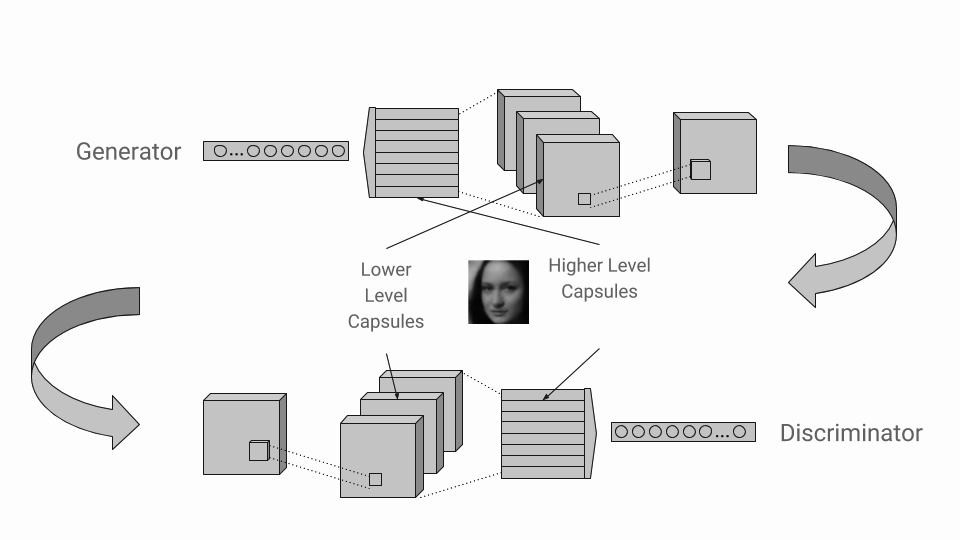
\includegraphics[width=1\textwidth]{images/methodology.png}
\caption{Proposed architecture}
\label{fig:capsgan}
\end{figure}

During the course of our research we were forced to conclude that building a CapsNet based generator was not feasible. A fundamental aspect of CapsNet is dynamic routing which is not possible to replicate in the generator, that is, dynamic routing cannot be inverted. Hence we implemented just the discriminator in CapsNet. 
\par\bigskip

We concentrated on four networks: DCGAN, WGAN, ACGAN and InfoGAN. Our training laboratory was Colloboratory - the cloud machine learning research platform. We trained each network individually for 20,000 epochs each. For our preliminary training we used the MNIST dataset. The MNIST dataset is a large dataset of handwritten digits commonly used for image processing training tasks. Each of the networks had it's discriminator augmented with the CapsNet code. The networks with the CapsNet discriminator were then individually trained on the same dataset, for 20,000 epochs each. Overall, it took us a few days to train all the networks and gather all the data.
\par\bigskip

\section{Network Architectures} % (fold)
\label{sec:network_architectures}
The following are the network architectures of the generator and the discriminator.

\subsection{Generator} % (fold)
\label{sub:generator}
\begin{lstlisting}[basicstyle=\scriptsize,language=Python]
_________________________________________________________________
Layer (type)                 Output Shape              Param #   
=================================================================
dense_5 (Dense)              (None, 8192)              827392    
_________________________________________________________________
reshape_1 (Reshape)          (None, 8, 8, 128)         0         
_________________________________________________________________
batch_normalization_3 (Batch (None, 8, 8, 128)         512       
_________________________________________________________________
up_sampling2d_1 (UpSampling2 (None, 16, 16, 128)       0         
_________________________________________________________________
conv2d_1 (Conv2D)            (None, 16, 16, 128)       147584    
_________________________________________________________________
activation_1 (Activation)    (None, 16, 16, 128)       0         
_________________________________________________________________
batch_normalization_4 (Batch (None, 16, 16, 128)       512       
_________________________________________________________________
up_sampling2d_2 (UpSampling2 (None, 32, 32, 128)       0         
_________________________________________________________________
conv2d_2 (Conv2D)            (None, 32, 32, 64)        73792     
_________________________________________________________________
activation_2 (Activation)    (None, 32, 32, 64)        0         
_________________________________________________________________
batch_normalization_5 (Batch (None, 32, 32, 64)        256       
_________________________________________________________________
up_sampling2d_3 (UpSampling2 (None, 64, 64, 64)        0         
_________________________________________________________________
conv2d_3 (Conv2D)            (None, 64, 64, 32)        18464     
_________________________________________________________________
activation_3 (Activation)    (None, 64, 64, 32)        0         
_________________________________________________________________
batch_normalization_6 (Batch (None, 64, 64, 32)        128       
_________________________________________________________________
conv2d_4 (Conv2D)            (None, 64, 64, 3)         867       
_________________________________________________________________
activation_4 (Activation)    (None, 64, 64, 3)         0         
=================================================================
Total params: 1,069,507
Trainable params: 1,068,803
Non-trainable params: 704
_________________________________________________________________
\end{lstlisting}
% subsection generator (end)

\subsection{Discriminator} % (fold)
\label{sub:discriminator}
\begin{lstlisting}[basicstyle=\scriptsize,language=Python]
____________________________________________________________________________________________
Layer (type)                    Output Shape         Param #     Connected to               
============================================================================================
input_1 (InputLayer)            (None, 64, 64, 3)    0                                      
____________________________________________________________________________________________
conv1 (Conv2D)                  (None, 56, 56, 256)  62464       input_1[0][0]              
____________________________________________________________________________________________
leaky_re_lu_1 (LeakyReLU)       (None, 56, 56, 256)  0           conv1[0][0]                
____________________________________________________________________________________________
batch_normalization_1 (BatchNor (None, 56, 56, 256)  1024        leaky_re_lu_1[0][0]        
____________________________________________________________________________________________
primarycap_conv2 (Conv2D)       (None, 24, 24, 256)  5308672     batch_normalization_1[0][0]
____________________________________________________________________________________________
primarycap_reshape (Reshape)    (None, 18432, 8)     0           primarycap_conv2[0][0]     
____________________________________________________________________________________________
primarycap_squash (Lambda)      (None, 18432, 8)     0           primarycap_reshape[0][0]   
____________________________________________________________________________________________
batch_normalization_2 (BatchNor (None, 18432, 8)     32          primarycap_squash[0][0]    
____________________________________________________________________________________________
flatten_1 (Flatten)             (None, 147456)       0           batch_normalization_2[0][0]
____________________________________________________________________________________________
uhat_digitcaps (Dense)          (None, 160)          23593120    flatten_1[0][0]            
____________________________________________________________________________________________
softmax_digitcaps1 (Activation) (None, 160)          0           uhat_digitcaps[0][0]       
____________________________________________________________________________________________
dense_1 (Dense)                 (None, 160)          25760       softmax_digitcaps1[0][0]   
____________________________________________________________________________________________
multiply_1 (Multiply)           (None, 160)          0           uhat_digitcaps[0][0]       
                                                                 dense_1[0][0]              
____________________________________________________________________________________________
leaky_re_lu_2 (LeakyReLU)       (None, 160)          0           multiply_1[0][0]           
____________________________________________________________________________________________
softmax_digitcaps2 (Activation) (None, 160)          0           leaky_re_lu_2[0][0]        
____________________________________________________________________________________________
dense_2 (Dense)                 (None, 160)          25760       softmax_digitcaps2[0][0]   
____________________________________________________________________________________________
multiply_2 (Multiply)           (None, 160)          0           uhat_digitcaps[0][0]       
                                                                 dense_2[0][0]              
____________________________________________________________________________________________
leaky_re_lu_3 (LeakyReLU)       (None, 160)          0           multiply_2[0][0]           
____________________________________________________________________________________________
softmax_digitcaps3 (Activation) (None, 160)          0           leaky_re_lu_3[0][0]        
____________________________________________________________________________________________
dense_3 (Dense)                 (None, 160)          25760       softmax_digitcaps3[0][0]   
____________________________________________________________________________________________
multiply_3 (Multiply)           (None, 160)          0           uhat_digitcaps[0][0]       
                                                                 dense_3[0][0]              
____________________________________________________________________________________________
leaky_re_lu_4 (LeakyReLU)       (None, 160)          0           multiply_3[0][0]           
____________________________________________________________________________________________
dense_4 (Dense)                 (None, 1)            161         leaky_re_lu_4[0][0]        
============================================================================================
Total params: 29,042,753
Trainable params: 29,042,225
Non-trainable params: 528
____________________________________________________________________________________________
\end{lstlisting}
% subsection discriminator (end)

% section network_architectures (end)

\section{Demonstration} % (fold)
\label{sec:demonstration}
The training of the models took place on Colaboratory, over Keras. Keras provided for a fast implementation of the code and high level abstraction. The output model was in the format of H5. This could not be directly used as part of semantic inpainting as semantic inpainting requires changing low level architectural details which Keras does not allow. Hence we converted the H5 model to TensorFlow protocol buffer, which is TensorFlow's model saving format, the code for which can be found in \ref{sub:converting_models}.
\par\bigskip

For the semantic inpainting, we take as input an image. The image is loaded onto a canvas with an ability to mask a part of the image. Once the mask is set, our processing starts. The following process is based on Raymond A. Yeh \textit{et al.} \cite{inpainting}
\par\bigskip

The masked image is a Hadamard product of the mask component, M, and the original input image, y. 
\begin{equation} \label{eqn:masked_image}
Masked Image = \bm{M} \odot\  \bm{y}
\end{equation}
\par\bigskip

Suppose we've found an image from the generator $G(\hat z)$ for some $\hat z$ that gives a reasonable reconstruction of the missing portions. The completed pixels $(1 - M) \odot G(\hat z)$ can be added to the original pixels to create the reconstructed image:
\begin{equation} \label{eqn:reconstructed_image}
\bm{x} \textsubscript{reconstructed} = \bm{M} \odot\  \bm{y} + (1 - \bm{M}) \odot \bm{G} (\hat z)
\end{equation}
\par\bigskip

Now all that is needed is to find a $G(\hat z)$ that does a good enough job of completing the image. We will consider a loss function, a smaller value of which means that z is more suitable for completion. The total loss function will be a sum of two loss functions: Contextual and Perceptual.

\subsection{Contextual Loss} % (fold)
\label{sub:contextual_loss}
To keep the same context as the input image, make sure the known pixel locations in the input image y are similar to the pixels in $G(z)$. We need to penalize $G(z)$ for not creating a similar image for the pixels that we know about. Formally, we do this by element-wise subtracting the pixels in $y$ from $G(z)$ and looking at how much they differ:
\begin{equation} \label{eqn:contextual_loss}
\bm{L}\textsubscript{contextual}(\bm{z}) = || \bm{M} \odot\  \bm{G(m)} + (1 - \bm{M}) \odot \bm{G} (\hat z) || \textsubscript{1}
\end{equation}
where $||x|| \textsubscript{1}=\sum \textsubscript{i} |x \textsubscript{i}|$ is the $l \textsubscript{1}$ norm of some vector $x$.

% subsection contextual_loss (end)

\subsection{Perceptual Loss} % (fold)
\label{sub:perceptual_loss}
To recover an image that looks real, let’s make sure the discriminator is properly convinced that the image looks real. We’ll do this with the same criterion used in training the network:
\begin{equation} \label{eqn:perceptual_loss}
\bm{L}\textsubscript{perceptual}(\bm{z}) = \bm{log} (1 - \bm{D}(\bm{G}(\bm{z})))
\end{equation}
% subsection perceptual_loss (end)

\subsection{Total Loss} % (fold)
\label{sub:total_loss}
We now find $\hat z$ with a combination of the contextual and perceptual losses:
\begin{equation} \label{eqn:total_loss}
\bm{L}(\bm{z}) = \bm{L}\textsubscript{contextual}(\bm{z}) + \lambda \bm{L}\textsubscript{perceptual}(\bm{z})
\end{equation}
\begin{equation} \label{eqn:minimization}
\hat z = arg \min_z \bm{L} (\bm{z})
\end{equation}

where $\lambda$ is a hyper-parameter that controls how important the contextual loss is relative to the perceptual loss. Then as before, the reconstructed image fills in the missing values of $\bm{y}$ with $\bm{G}(\bm{z})$:
\begin{equation} \label{eqn:reconstructed_image_final}
\bm{x} \textsubscript{reconstructed} = \bm{M} \odot\  \bm{y} + (1 - \bm{M}) \odot \bm{G} (\hat z)
\end{equation}
% subsection total_loss (end)

\subsection{Projected Gradient Descent} % (fold)
\label{sub:projected_gradient_descent}
	For minimizing the loss function we use projected gradient descent. Its different from gradient descent in the sense, at a basic level, projected gradient descent is just a more general method for solving a more general problem. Gradient descent minimizes a function by moving in the negative gradient direction at each step. There is no constraint on the variable. 
\begin{equation} \label{eqn:gradient_descent}
\text{Problem 1:} \min_x f(x)
$$
$$
x_{k+1} = x_k - t_k \nabla f(x_k)
\end{equation}

On the other hand, projected gradient descent minimizes a function subject to a constraint. At each step we move in the direction of the negative gradient, and then "project" onto the feasible set.

\begin{equation} \label{eqn:projected_gradient_descent}
\text{Problem 2:} \min_x f(x) \text{ subject to } x \in C
$$
$$
y_{k+1} = x_k - t_k \nabla f(x_k)
$$
$$
x_{k+1} = \text{arg} \min_{x \in C} \|y_{k+1}-x\| 
\end{equation}

% subsection projected_gradient_descent (end)

% section demonstration (end)
\par

\part*{Chapter 7\\ Code Snippets}
{\chapter{Code snippets}\label{ch:scope}}
\epigraph{\textit{\normalsize “By far the greatest danger of Artificial Intelligence is that people conclude too early that they understand it.”}}{\textit{ \normalsize Eliezer Yudkowsky,\\ Machine Intelligence Research Institute}}

\section{Building Generator} % (fold)
\label{sec:building_generator}
\begin{lstlisting}[basicstyle=\scriptsize,language=Python]
def build_generator(self):

    model = Sequential()

    model.add(Dense(128 * 8 * 8, activation="relu", input_shape=(self.latent_dim,)))
    model.add(Reshape((8, 8, 128)))
    model.add(BatchNormalization(momentum=0.8))
    model.add(UpSampling2D())
    model.add(Conv2D(128, kernel_size=3, padding="same"))
    model.add(Activation("relu"))
    model.add(BatchNormalization(momentum=0.8))
    model.add(UpSampling2D())
    model.add(Conv2D(64, kernel_size=3, padding="same"))
    model.add(Activation("relu"))
    model.add(BatchNormalization(momentum=0.8))
    model.add(UpSampling2D())
    model.add(Conv2D(32, kernel_size=3, padding="same"))
    model.add(Activation("relu"))
    model.add(BatchNormalization(momentum=0.8))
    model.add(Conv2D(self.channels, kernel_size=3, padding="same"))
    model.add(Activation("tanh"))

    model.summary()

    noise = Input(shape=(self.latent_dim,))
    img = model(noise)

    return Model(noise, img)

\end{lstlisting}
% section building_generator (end)
\par

\part*{Chapter 8\\ Execution and Results}
\chapter{Execution and Results}\label{ch:execandresults}
\epigraph{\textit{ \normalsize“ We dont have better algorithms, we just have more data”}}{\normalsize\textit{Peter Norvig,\\ Director of Research at Google Inc.}}

\section{Training} % (fold)
\label{sec:training}

% section training (end)
Our research consisted of four networks: ACGAN, DCGAN, InfoGAN and WGAN. Each of the networks was trained for 20,000 epochs each. The training period for the individual networks took anywhere between a few hours and a couple of days. For each network, we logged a few key metrics, mainly the Generator Loss (GLoss), Discriminator Loss (DLoss) and the Accuracy (Acc). 
\par\bigskip
Below we show graphically the performance of the (four) classical networks as compared to the CapsNet discriminator augmented networks.

\begin{figure}[H]
    \centering
    \subfloat[Classical ACGAN]{{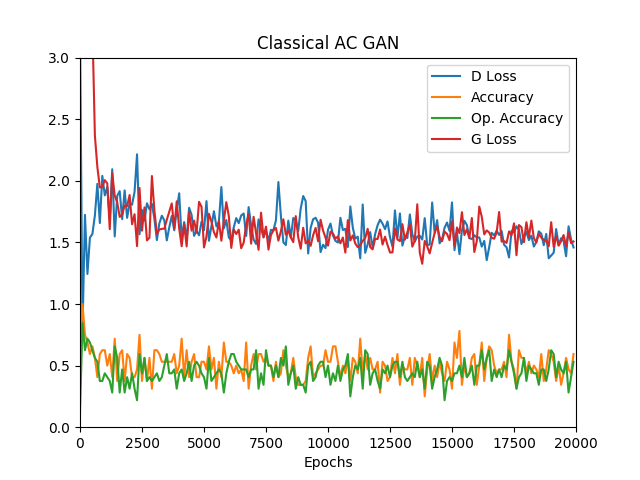
\includegraphics[width=.45\linewidth]{images/plots/classacgan.png} }}%
    \qquad
    \subfloat[CapsNet augmented ACGAN]{{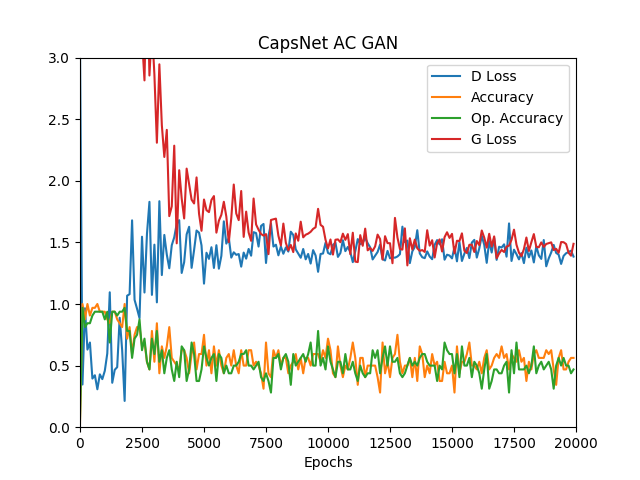
\includegraphics[width=.45\linewidth]{images/plots/capsacgan.png} }}%
    \caption{ACGAN metrics}%
    \label{fig:acgan}%
\end{figure}

\begin{figure}[H]
    \centering
    \subfloat[Classical DCGAN]{{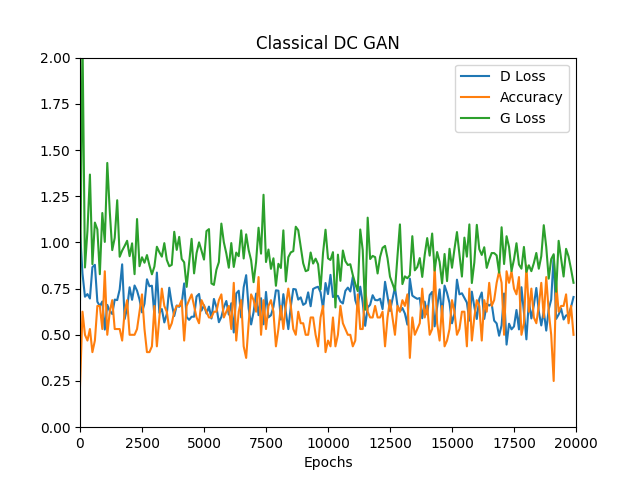
\includegraphics[width=.45\linewidth]{images/plots/classdcgan.png} }}%
    \qquad
    \subfloat[CapsNet augmented DCGAN]{{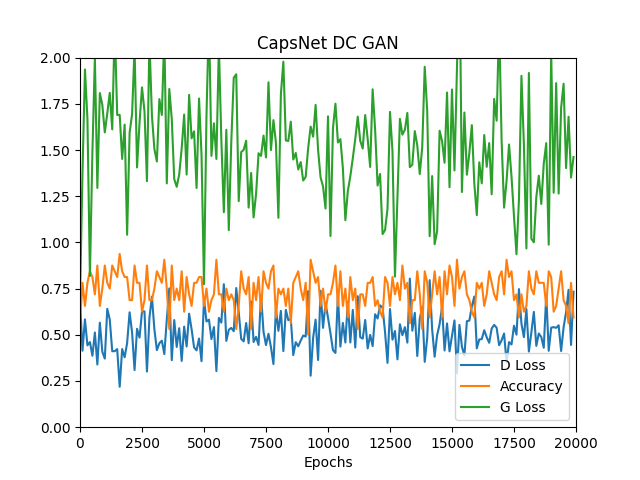
\includegraphics[width=.45\linewidth]{images/plots/capsdcgan.png} }}%
    \caption{DCGAN metrics}%
    \label{fig:dcgan}%
\end{figure}

\begin{figure}[H]
    \centering
    \subfloat[Classical InfoGAN]{{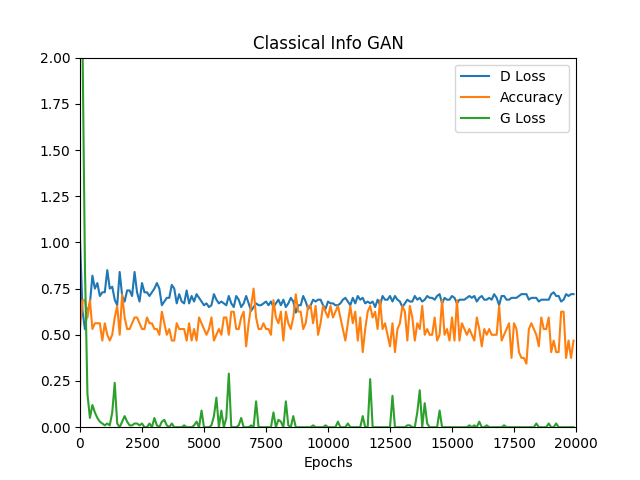
\includegraphics[width=.45\linewidth]{images/plots/classinfogan.png} }}%
    \qquad
    \subfloat[CapsNet augmented InfoGAN]{{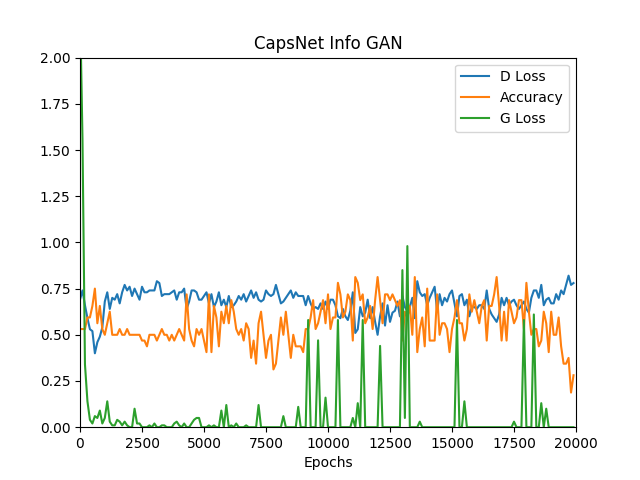
\includegraphics[width=.45\linewidth]{images/plots/capsinfogan.png} }}%
    \caption{InfoGAN metrics}%
    \label{fig:infogan}%
\end{figure}

\begin{figure}[H]
    \centering
    \subfloat[Classical WGAN]{{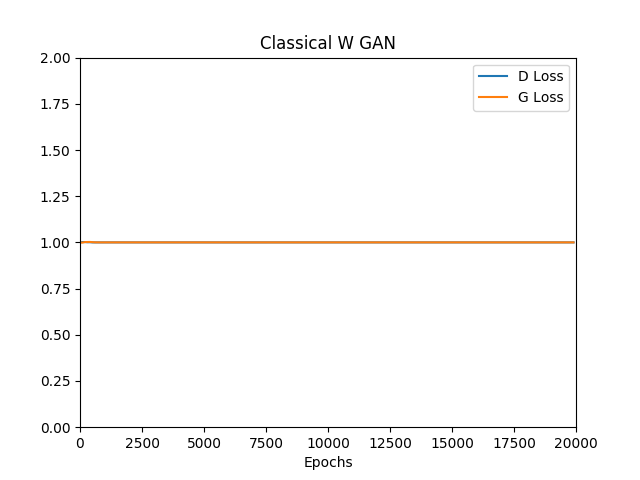
\includegraphics[width=.45\linewidth]{images/plots/classwgan.png} }}%
    \qquad
    \subfloat[CapsNet augmented WGAN]{{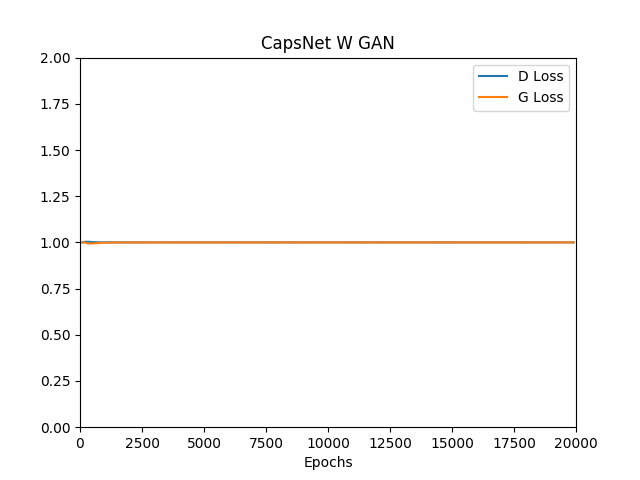
\includegraphics[width=.45\linewidth]{images/plots/capswgan.png} }}%
    \caption{WGAN metrics}%
    \label{fig:wgan}%
\end{figure}

The metrics of WGAN are at a smaller scale, so below is a comparison at the lower scale.

\begin{figure}[H]
    \centering
    \subfloat[Classical WGAN]{{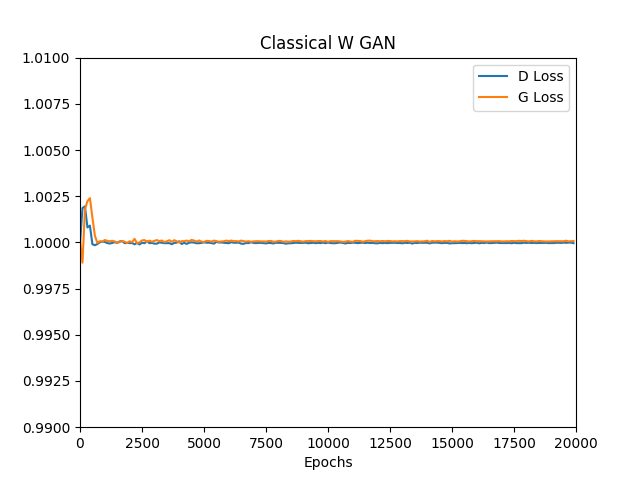
\includegraphics[width=.45\linewidth]{images/plots/classwgan-zoomed.png} }}%
    \qquad
    \subfloat[CapsNet augmented WGAN]{{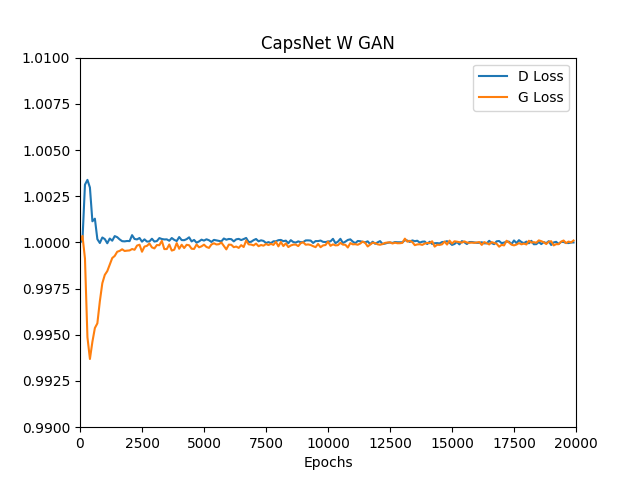
\includegraphics[width=.45\linewidth]{images/plots/capswgan-zoomed.png} }}%
    \caption{WGAN metrics - zoomed}%
    \label{fig:wgan}%
\end{figure}
\par\bigskip

A preliminarily analysis of the data shows us that our CapsNet augmented networks, hence-forth referred to as the network name prefixed with "Caps", perform comparably with the classical architectures. 
\par\bigskip

Under ACGAN we see that CapsACGAN starts off with very high variance in GLoss and DLoss. Over the course of 20,000 epochs, the variance gradually reduces to match the Classical ACGAN metrics at the end. Accuracy of CapsACGAN, on the other hand, quickly stabilizes to meet classical ACGAN metrics. As a side note, ACGAN was the fastest trained network, taking roughly three hours to complete 20,000 epochs.
\par\bigskip

DCGAN and InfoGAN are interesting in the sense that they show a remarkable shift in the GLoss metric. Even though it seems as if augmenting DCGAN with CapsNet discriminator leads to increase in GLoss, a closer look reveals that increased variation leads to faster learning of the generator network. Accuracy and DLoss follow their classical counterpart closely.
\par\bigskip

WGAN happens to be the best and state-of-the-art. Consequently, the variance in the metrics were at a much smaller scale, that is, the network is designed to be more stabilized and balanced but this also leads to slower learning, we can see that adding CapsNet discriminator speeds this up by adding slightly more variance while the network is still balanced. We had to zoom-in to notice the difference between the metrics. We see that an initial burst of high variance quickly stabilizes to trace a path closely matching the classical architecture.
\par\bigskip

\section{Generation} % (fold)
\label{sec:generation}
At the end of every epoch we saved the outputs of the generator. Here we show the outputs of generator of four networks after 20,000 epochs for comparison.
\begin{figure}[H]
    \centering
    \subfloat[Classical ACGAN]{{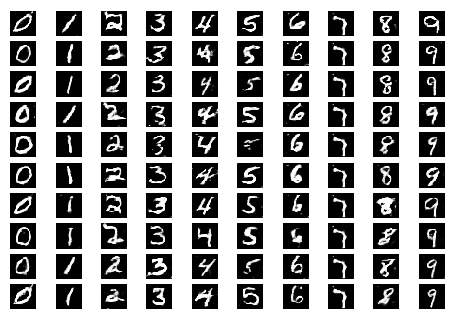
\includegraphics[width=.5\linewidth]{images/generation_outputs/acgan.png} }}%
    \subfloat[CapsNet augmented ACGAN]{{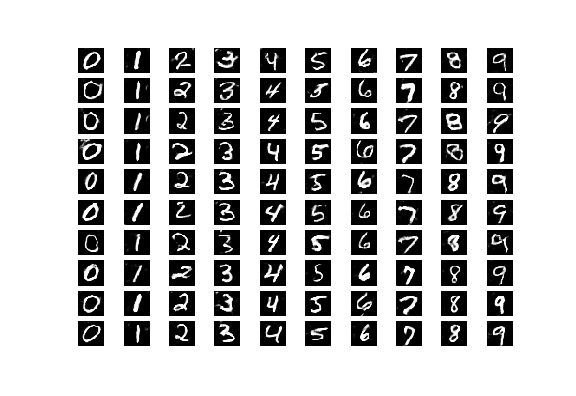
\includegraphics[width=.5\linewidth]{images/generation_outputs/acgan_caps.png} }}%
    \caption{ACGAN outputs}%
    \label{fig:acgan_gen}%
\end{figure}
As expected from the metrics the ACGAN and CapsACGAN produce very similar outputs.
\begin{figure}[H]
    \centering
    \subfloat[Classical DCGAN]{{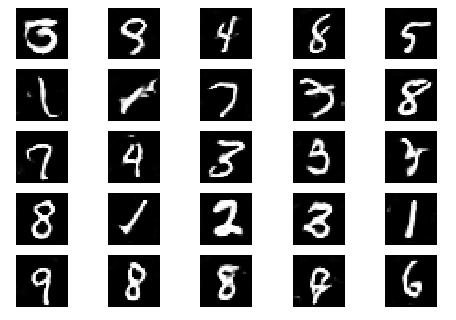
\includegraphics[width=.45\linewidth]{images/generation_outputs/dcgan.png} }}%
    \qquad
    \subfloat[CapsNet augmented DCGAN]{{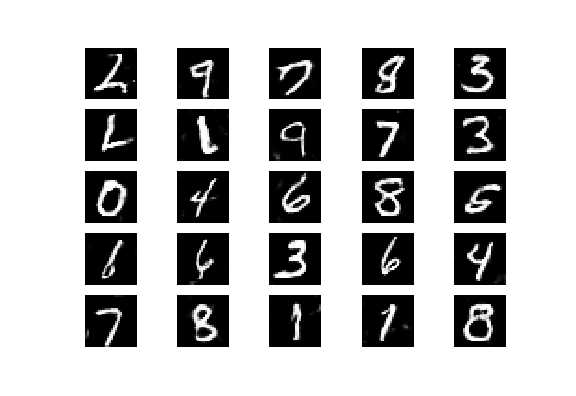
\includegraphics[width=.45\linewidth]{images/generation_outputs/dcgan_caps.png} }}%
    \caption{DCGAN outputs}%
    \label{fig:dcgan_gen}%
\end{figure}
The outputs of DCGAN and CapsDCGAN are almost indistinguishable but a closer look reveals that CapsDCGAN produces more clear outputs and more percentage of CapsDCGAN outputs look real.

\begin{figure}[H]
    \centering
    \subfloat[Classical InfoGAN]{{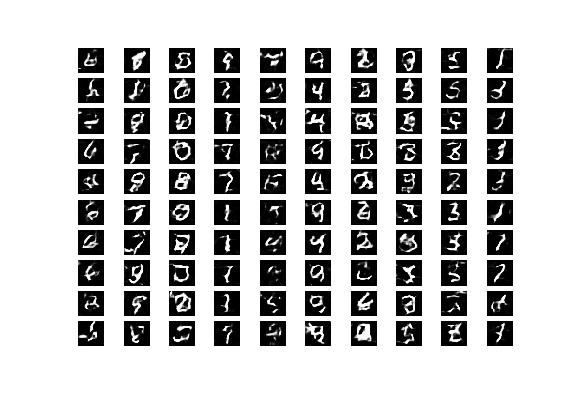
\includegraphics[width=.5\linewidth]{images/generation_outputs/infogan.png} }}%
    \subfloat[CapsNet augmented InfoGAN]{{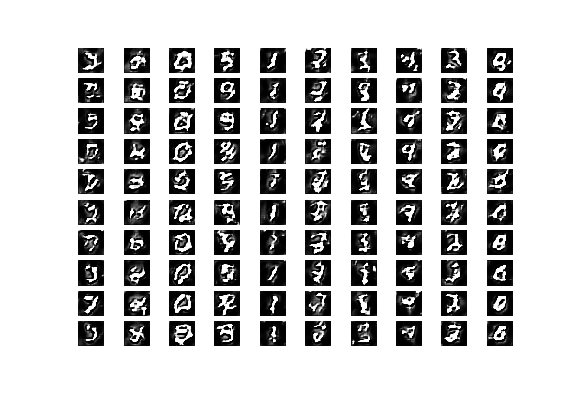
\includegraphics[width=.5\linewidth]{images/generation_outputs/infogan_caps.png} }}%
    \caption{InfoGAN outputs}%
    \label{fig:infogan_gen}%
\end{figure}
Even though the CapsInfoGAN output looks structurally more better and has learned faster but it is more noisier than that of the InfoGAN.
\begin{figure}[H]
    \centering
    \subfloat[Classical WGAN]{{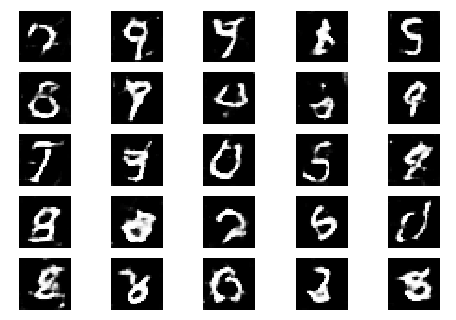
\includegraphics[width=.45\linewidth]{images/generation_outputs/wgan.png} }}%
    \qquad
    \subfloat[CapsNet augmented WGAN]{{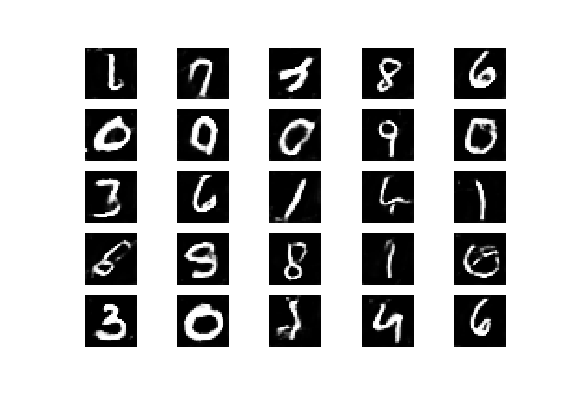
\includegraphics[width=.45\linewidth]{images/generation_outputs/wgan_caps.png} }}%
    \caption{WGAN outputs}%
    \label{fig:wgan_gen}%
\end{figure}
Finally in the WGAN outputs we can clearly see that CapsWGAN produces clear and better outputs, hence has learned more quickly than the WGAN. 

% section generation (end)

\section{Demonstration} % (fold)
\label{sec:demonstration}

Initially, for demonstration of semantic in-painting, we used the MNIST model of CapsDCGAN that we used in the previous sections. We had promising results as seen in the figure \ref{fig:mnist_examples}.

\begin{figure}[H]
    \centering
    \subfloat{{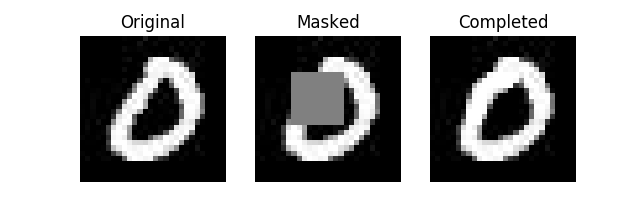
\includegraphics[width=.5\linewidth]{images/completion_outputs/0_1.png} }}%
    \subfloat{{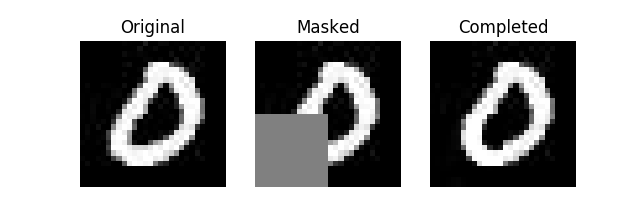
\includegraphics[width=.5\linewidth]{images/completion_outputs/0_2.png} }}%
    \\
    \centering
    \subfloat{{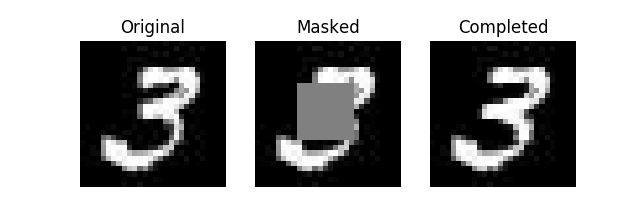
\includegraphics[width=.5\linewidth]{images/completion_outputs/3_1.png} }}%
    \subfloat{{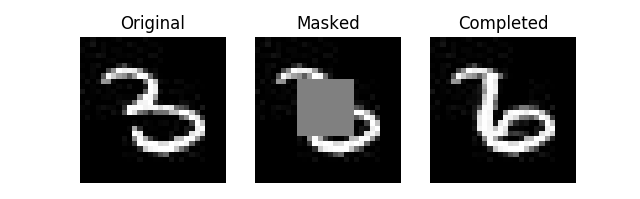
\includegraphics[width=.5\linewidth]{images/completion_outputs/3_2.png} }}%
    \\
    \centering
    \subfloat{{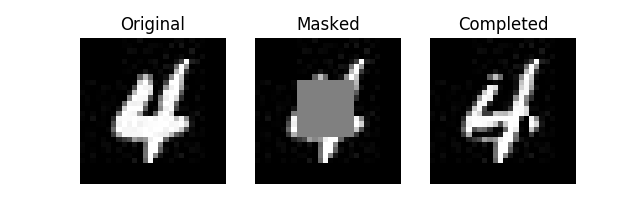
\includegraphics[width=.5\linewidth]{images/completion_outputs/4.png} }}%
    \subfloat{{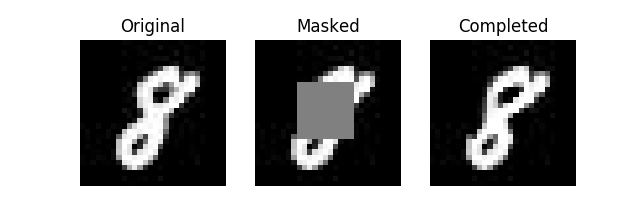
\includegraphics[width=.5\linewidth]{images/completion_outputs/8_1.png} }}%
    \\
    \centering
    \subfloat{{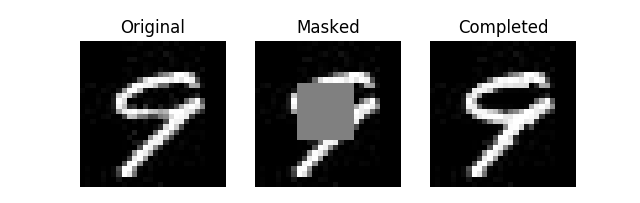
\includegraphics[width=.5\linewidth]{images/completion_outputs/9_1.png} }}%
    \caption{MNIST examples}%
    \label{fig:mnist_examples}%
\end{figure}
For the completion of faces however the process was more complex. We initially trained CapsDCGAN on LFW dataset \cite{lfw} for 50 epochs. Since LFW contains only 13,233 images, the model suffered from low generalization. So we decided to use the larger CelebA dataset \cite{celeba} for training. CelebA consists of 202,599 images of 10,177 celebrities. We trained CapsDCGAN on CelebA for only 9 epochs and still obtained realistic images. The following are the completion outputs from CelebA model in figure \ref{fig:face_examples}.
\begin{figure}[H]
    \centering
    \subfloat{{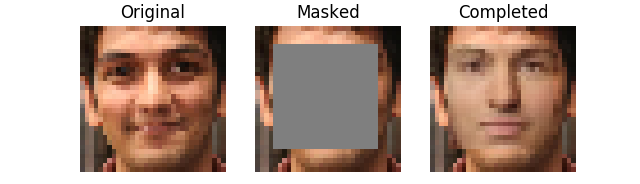
\includegraphics[width=.5\linewidth]{images/completion_outputs/Figure_10.png} }}%
    \subfloat{{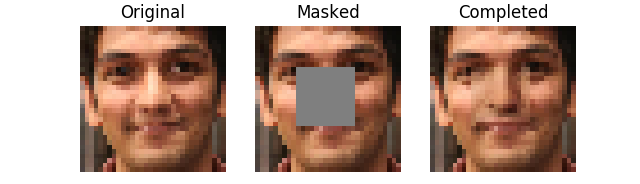
\includegraphics[width=.5\linewidth]{images/completion_outputs/Figure_11.png} }}%
    \\
    \centering
    \subfloat{{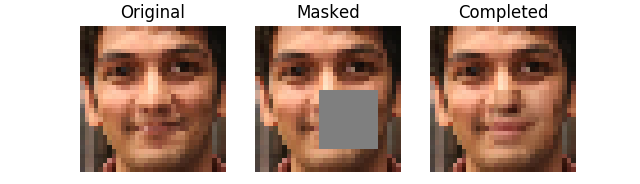
\includegraphics[width=.5\linewidth]{images/completion_outputs/Figure_12.png} }}%
    \subfloat{{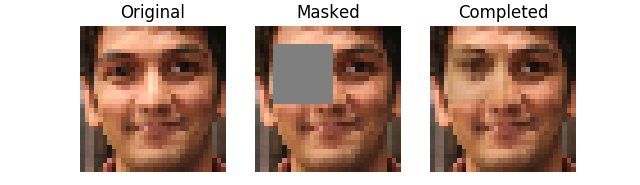
\includegraphics[width=.5\linewidth]{images/completion_outputs/Figure_13.png} }}%
    \\
    \centering
    \subfloat{{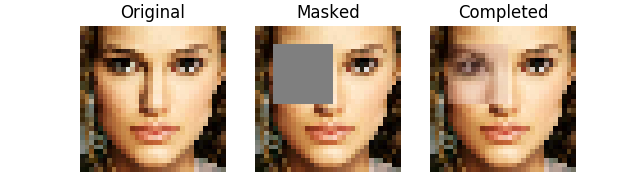
\includegraphics[width=.5\linewidth]{images/completion_outputs/Figure_14.png} }}%
    \subfloat{{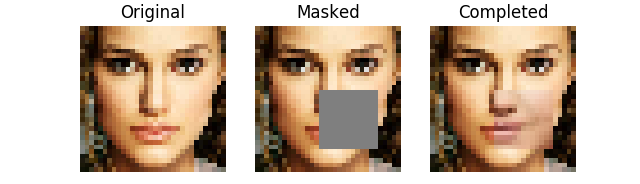
\includegraphics[width=.5\linewidth]{images/completion_outputs/Figure_15.png} }}%
    \\
    \centering
    \subfloat{{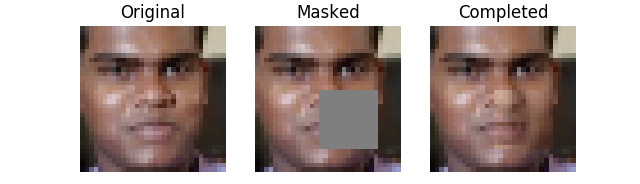
\includegraphics[width=.5\linewidth]{images/completion_outputs/Figure_16.png} }}%
    \subfloat{{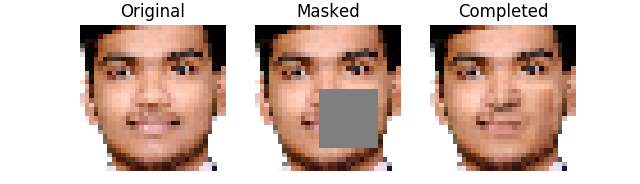
\includegraphics[width=.5\linewidth]{images/completion_outputs/Figure_17.png} }}%
    \\
    \centering
    \subfloat{{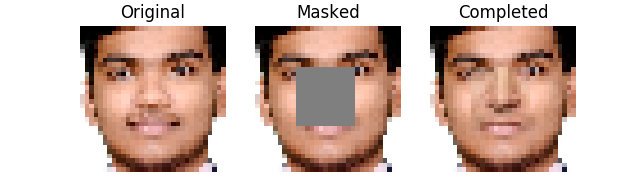
\includegraphics[width=.5\linewidth]{images/completion_outputs/Figure_18.png} }}%
    \subfloat{{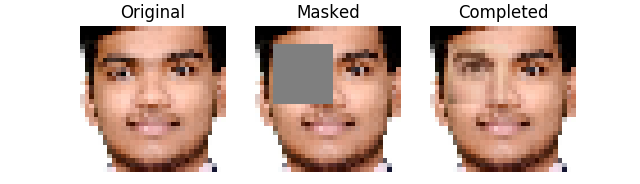
\includegraphics[width=.5\linewidth]{images/completion_outputs/Figure_19.png} }}%
    \\
    \centering
    \subfloat{{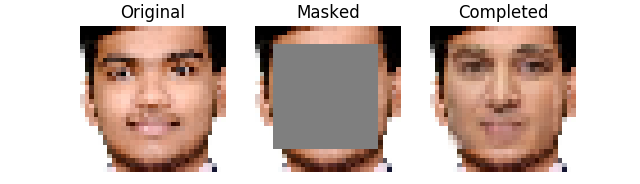
\includegraphics[width=.5\linewidth]{images/completion_outputs/Figure_20.png} }}%

    \caption{Face examples}%
    \label{fig:face_examples}%
\end{figure}


\par

\part*{Chapter 9\\ Conclusion}
\chapter{Conclusion}\label{ch:conclusion}
\epigraph{\textit{\Large “A year spent in artificial intelligence is enough to make one believe in God”}}{\textit{ \large Alan Perlis,\\ First Turning award recepient}}
During the course of this project, we wish to replicate the results of the existing state-of-the-art in Generative Models. Using this as a stepping stone, we would like to incorporate a hitherto unexplored option in CapsNet for Generative Models. Our motivating assumption is that CapsNet would provide a performance improvement.We base this on the idea that it is more capable of understanding the variances in objects. This in turn should lead to lower data requirements during training of the model and consequently lower power consumption. 

\par\bigskip We wish to provide a comparison between our novel CapsNet-based approach and other implementations of GAN for the same task. We would like to implement a proof of concept by developing a application to complete incomplete images of human faces. This could later on be used in enhancement of hazy CCTV footage to identify individuals, which would be immensely helpful to law enforcement personnel.

\vspace{200px}
\centering
\textbf{Head of Department}
\vspace{50px}
\flushleft\textbf{Project Guide}\hfill\textbf{Project Coordinator}
\par\clearpage
\bibliography{ref}{}
\bibliographystyle{plainyr-rev}
\par
\end{document}
